%%%%%%%%%%%%%%%%%%%%%%%%%%%%%%%%%%%%%%%%%
% Professional Newsletter Template
% LaTeX Template
% Version 1.0 (09/03/14)
%
% Created by:
% Bob Kerstetter (https://www.tug.org/texshowcase/) and extensively modified by:
% Vel (vel@latextemplates.com)
% 
% This template has been downloaded from:
% http://www.LaTeXTemplates.com
%
% License:
% CC BY-NC-SA 3.0 (http://creativecommons.org/licenses/by-nc-sa/3.0/)
%
%%%%%%%%%%%%%%%%%%%%%%%%%%%%%%%%%%%%%%%%%

\documentclass[9pt]{extarticle} % The default font size is 10pt; 11pt and 12pt are alternatives

%%%%%%%%%%%%%%%%%%%%%%%%%%%%%%%%%%%%%%%%%
% Professional Newsletter Template
% Structural Definitions File
% Version 1.0 (09/03/14)
%
% Created by:
% Vel (vel@latextemplates.com)
% 
% This file has been downloaded from:
% http://www.LaTeXTemplates.com
%
% License:
% CC BY-NC-SA 3.0 (http://creativecommons.org/licenses/by-nc-sa/3.0/)
%
%%%%%%%%%%%%%%%%%%%%%%%%%%%%%%%%%%%%%%%%%

%----------------------------------------------------------------------------------------
%	REQUIRED PACKAGES
%----------------------------------------------------------------------------------------

\usepackage{listings}
\usepackage{graphicx} % Required for including images
\usepackage{microtype} % Improved typography
\usepackage{multicol} % Used for the two-column layout of the document
\usepackage{booktabs} % Required for nice horizontal rules in tables
\usepackage{wrapfig} % Required for in-line images
\usepackage{float} % Required for forcing figures not to float with the [H] parameter
\usepackage[utf8]{inputenc}
\usepackage{fancyhdr}

%------------------------------------------------
% Fonts

\usepackage{charter} % Use the Charter font as the main document font
\usepackage{courier} % Use the Courier font for \texttt (monospaced) only
\usepackage[T1]{fontenc} % Use T1 font encoding

%------------------------------------------------
% List Separation

\usepackage{enumitem} % Required to customize the list environments
\setlist{noitemsep,nolistsep} % Remove spacing before, after and within lists for a compact look

%------------------------------------------------
% Figure and Table Caption Styles

\usepackage{caption} % Required for changing caption styles
\captionsetup[table]{labelfont={bf,sf},labelsep=period,justification=justified} % Specify the table caption style
\captionsetup[figure]{labelfont={sf,bf},labelsep=period,justification=justified, font=small} % Specify the figure caption style
\setlength{\abovecaptionskip}{10pt} % Whitespace above captions

%------------------------------------------------
% Spacing Between Paragraphs

\makeatletter
\usepackage{parskip}
\setlength{\parskip}{6pt}
\newcommand{\@minipagerestore}{\setlength{\parskip}{6pt}}
\makeatother

%----------------------------------------------------------------------------------------
%	PAGE MARGINS AND SPACINGS
%----------------------------------------------------------------------------------------

\textwidth = 7 in % Text width
\textheight = 10 in % Text height
\oddsidemargin = -18pt % Left side margin on odd pages
\evensidemargin = -18pt % Left side margin on even pages
\topmargin = -36pt % Top margin
\headheight = 0pt % Remove the header by setting its space to 0
\headsep = 0pt % Remove the space between the header and top of the page
\parskip = 2pt % Space between paragraph
\parindent = 0.0in % Paragraph indentation
\pagestyle{empty} % Disable page numbering

%----------------------------------------------------------------------------------------
%	COLORS
%----------------------------------------------------------------------------------------

\usepackage[dvipsnames,svgnames]{xcolor} % Required to specify custom colors

\definecolor{altncolor}{rgb}{.8,0,0} % Dark red
%\definecolor{altncolor}{rgb}{.2,.4,.8} % Dark blue
%\definecolor{altncolor}{rgb}{.84,.16,.16} % Red

\usepackage[colorlinks=true, linkcolor=altncolor, anchorcolor=altncolor, citecolor=altncolor, filecolor=altncolor, menucolor=altncolor, urlcolor=altncolor]{hyperref} % Use the color defined above for all links

%----------------------------------------------------------------------------------------
%	BOX STYLES
%----------------------------------------------------------------------------------------

\usepackage[framemethod=TikZ]{mdframed}% Required for creating boxes
\mdfdefinestyle{sidebar}{
    linecolor=black, % Outer line color
    outerlinewidth=0.5pt, % Outer line width
    roundcorner=0pt, % Amount of corner rounding
    innertopmargin=10pt, % Top margin
    innerbottommargin=10pt, % Bottom margin
    innerrightmargin=10pt, % Right margin
    innerleftmargin=10pt, % Left margin
    backgroundcolor=white, % Box background color
    frametitlebackgroundcolor=white, % Title background color
    frametitlerule=false, % Title rule - true or false
    frametitlerulecolor=white, % Title rule color
    frametitlerulewidth=0.5pt, % Title rule width
    frametitlefont=\Large, % Title heading font specification
    font=\small
}

\mdfdefinestyle{intextbox}{
    linecolor=black, % Outer line color
    outerlinewidth=0.5pt, % Outer line width
    roundcorner=10pt, % Amount of corner rounding
    innertopmargin=7pt, % Top margin
    innerbottommargin=7pt, % Bottom margin
    innerrightmargin=7pt, % Right margin
    innerleftmargin=7pt, % Left margin
    backgroundcolor=white, % Box background color
    frametitlebackgroundcolor=white, % Title background color
    frametitlerule=false, % Title rule - true or false
    frametitlerulecolor=white, % Title rule color
    frametitlerulewidth=0.5pt, % Title rule width
    frametitlefont=\Large % Title heading font specification
}

%----------------------------------------------------------------------------------------
%	HEADING STYLE
%----------------------------------------------------------------------------------------

\newcommand{\heading}[2]{ % Define the \heading command
\vspace{#2} % White space above the heading
{\begin{center}\Large\textbf{#1}\end{center}} % The heading style
\vspace{#2} % White space below the heading
}

\newcommand{\BackToContents}{\hyperlink{contents}{{\small Back to Contents}}} % Define a command for linking back to the contents of the newsletter % Include the document which specifies all packages and structural customizations for this template

\begin{document}

%--------------------------------------------------------------------------------
% HEADER DETAILS
%--------------------------------------------------------------------------------

\pagestyle{fancy}
\fancyhf{}
\chead{segfault@csh.rit.edu}
\rhead{\today}
\lhead{Volume XLVIII Issue \#11}
\addtolength\footskip{-15px}
\cfoot{"Node is faster since it does not have to deal with thread switching"
  - Andrew Wetmore (awetmore)}

%----------------------------------------------------------------------------------------
%	HEADER IMAGE
%----------------------------------------------------------------------------------------

\begin{figure}[H]
\centering\vspace{0.5cm}
\includegraphics[width=0.8\linewidth]{imgs/segfault.png}
\end{figure}

%--------------------------------------------------------------------------------
% HEADER QUOTE
%--------------------------------------------------------------------------------

\vspace{-15px}
\begin{quote}
\centering
\textbf{\textit{Batman for Chairman 2016 - 2017}}
\end{quote}
\vspace{10px}

%----------------------------------------------------------------------------------------
%	SIDEBAR - FIRST PAGE
%----------------------------------------------------------------------------------------

\vspace{-0.5cm}\begin{minipage}[t]{.35\linewidth} % Mini page taking up 35% of the actual page
\begin{mdframed}[style=sidebar,frametitle={}] % Sidebar box

%-----------------------------------------------------------

\hypertarget{contents}{\textbf{{\large This week on floor\ldots}}} % \hypertarget provides a label to reference using \hyperlink{label}{link text}
\begin{itemize}
\item \hyperlink{firstnews}{B-Trees}
\item \hyperlink{secondnews}{Software Engineer Translator}
\end{itemize}

\centerline {\rule{.75\linewidth}{.25pt}} % Horizontal line

%-----------------------------------------------------------

\textbf{Notable Upcoming Events:}
\begin{enumerate}[leftmargin=0.2cm]
\item \textbf{Super Game Jam Showing} May 4, 10:30pm \\
  Come join Zach and Noah for tons of fun!!
  \\
\item \textbf{RHA Tie-Dye Carnival} May 6, 2:00pm \\
  Come join the RHA for tie-dying and food.
  \\
\item \textbf{Insights Weekend} May 6 - 8 \\
  \\
\item \textbf{ImagineRIT} May 7, 10:00am \\
  \\
\item \textbf{IronChef CSH} \\
  CSH 1st annual cook-off!!
  \\
\item \textbf{Graduation Party} May 8, 1:00pm \\
  This will be hosted in AO55
  \\
\end{enumerate}

%-----------------------------------------------------------


\textbf{<TITLE>} \\
<SHORT SECTION>
\\

%-----------------------------------------------------------

\captionof*{table}{Voting Results}
\begin{tabular}{lcr}

Vote & Cost & Result \\
\midrule
<NAME> & \$<MONEY> & <STATUS> \\
\bottomrule
\end{tabular}

%-----------------------------------------------------------

\end{mdframed}
\end{minipage}\hfill % End the sidebar mini page 
%
%----------------------------------------------------------------------------------------
%	MAIN BODY - FIRST PAGE
%----------------------------------------------------------------------------------------
%
\begin{minipage}[t]{.61\linewidth} % Mini page taking up 61% of the actual page
\vspace{-0.4cm}
\hypertarget{firstnews}{\heading{B-Trees}{6pt}}
 
A b-tree is a type of self-balancing tree data structure that is heavily used in databases and
compute clusters. It is a type of binary search tree but it differs in that a node can have more
than 2 children. In fact, it has as many children as it can so that they all fit into a block on
disk. This way all of the children are read into memory with only 1 read. This makes it so that
they are optimized for systems that read and write large blocks of data, aka databases.

They wre introduced in 1907, and are still found in almost all major system today. They remain
to this date the standard way to implement on-disk indexes for almost all major relational
databases. Traditionally b-trees break each node into blocks of 4KB of size, due to the average
block size on-disk. Most of the data is stored on disk so that it can handle more than the size
of the memory on the machine. It takes advantage of the system's page cache to keep the most use
nodes in memory.

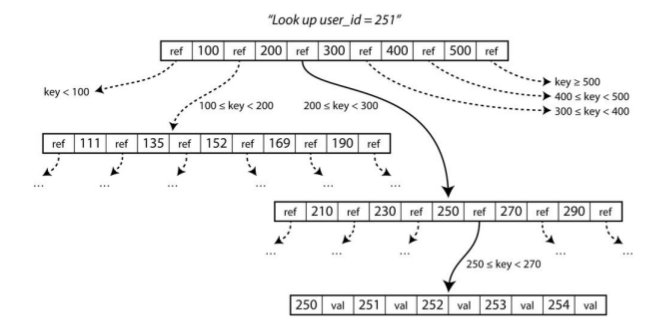
\includegraphics[width=0.8\linewidth]{imgs/b-tree.png}

One page is designated as the root node for the b-tree. The first step is to pull that node from
disk. It is normally located in memory already so the cost is very cheap. This node contains k
children references and the range of nodes that each is responsible for. You determine which
child you want to visit and repeat the process with reading it from disk. This process is designed
to do as little disk IO as possible.

%-----------------------------------------------------------

\hypertarget{secondnews}{\heading{Software Engineer Translator}{6pt}}

\textbf{What is said:} This is a horrible hack \\
\textbf{What it means:} This is a something that I did not write

\textbf{What is said:} It's broken \\
\textbf{What it means:} There are bugs in your code

\textbf{What is said:} It has a few issues \\
\textbf{What it means:} There are bugs in my code

\textbf{What is said:} It is self-documenting \\
\textbf{What it means:} My code doesn't have comments

\textbf{What is said:} emacs is better than vim \\
\textbf{What it means:} It's too peaceful, let's start a flame war

\textbf{What is said:} vim is better than emacs \\
\textbf{What it means:} It's too peaceful, let's start a flame war

\textbf{What is said:} Legacy code \\
\textbf{What it means:} It works, but no ones knows how

\end{minipage} % End the main body - first page mini page

\end{document} 
